%%%%%%
% OS %
%%%%%%

\section{Struktura OS -- systémové jádro, monolitický systém, architektura klient-server, virtuální stroje}
\label{kernel}

Operační systém si lze zjednodušeně představit jako program skládající se z~\emph{jádra} (\emph{kernel}) a~\emph{systémových programů}. Systémové programy jsou takové programy, které poskytují prostředí pro~spouštění a~běh \emph{aplikačních programů} (které nejsou součástí OS). Dále pak systémová volání fungují jako jakési API~pro~systémové programy, aby mohly volat funkce z~jádra (toto např. umožňuje čtení ze~souborů%
\footnote{Čtení ze~souboru probíhá pomocí systémového volání \texttt{open}, kde můžeme nastavovat různé možnosti, jako \texttt{O\_APPEND}, \texttt{O\_CREAT}.}%
 nebo jejich vytváření%
 \footnote{Soubor lze vytvořit například pomocí systémového volání \emph{open} s~možností \texttt{O\_CREAT}, která soubor vytvoří pokud neexistuje.}%
 ).

\begin{enumerate}
	\item Systémové programy -- knihovny
	\item Aplikační programy -- prohlížeč, textový editor, apod.
\end{enumerate}

\begin{figure}[ht]
	\centering
	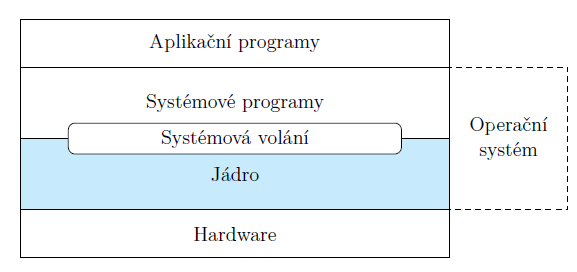
\includegraphics[scale=1]{images/OS_kernel_apps.png}
	\caption{Jádro a~aplikace}
	\label{OS_kernel_apps}
\end{figure}

V~operačních systémech zpravidla rozlišujeme dva základní režimy operací:

\begin{enumerate}
	\item režim jádra tj. privilegovaný/systémový režim
	\item uživatelský režim tj. neprivilegovaný režim
\end{enumerate}

V~uživatelském režimu běží všechny aplikace krom jádra (viz otázku \ref{procesy}).

\subsection{Monolitický systém}

Jak již napovídá samotný název, \emph{monolitický systém} je systém který nemá skoro žádnou strukturu. Jádro je pouze souhrn procedur, které se navzájem volají. Tento druh jádra vzniká kompilací zdrojových kódů na~objektové soubory (končící na~\texttt{.o}), tyto objektové soubory jsou potom \emph{svázány}/\emph{spojeny} v~tzv. \emph{linkeru} do~jednoho spustitelného souboru. Zde vyplývá na~povrch první značná nevýhoda monolitických jader: při~jakékoliv změně v~jádře je třeba jej kompletně překompilovat.

\begin{figure}[ht]
	\centering
	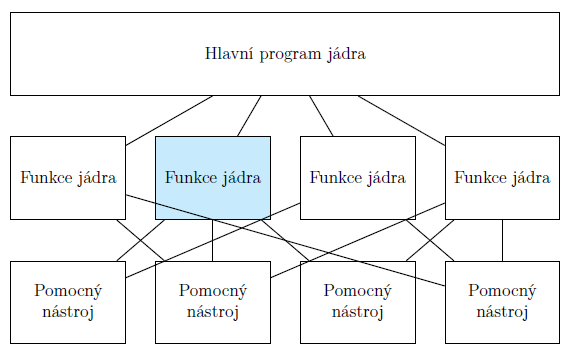
\includegraphics[scale=1]{images/OS_mono_kernel.png}
	\caption{Monolitické jádro}
	\label{OS_mono_kernel}
\end{figure}

I~když bylo řečeno, že monolitický systém vlastně žádnou strukturu nemá, není to zcela pravda, jak lze vidět z~obrázku \ref{OS_mono_kernel}: obsahuje hlavní program volající vyžádanou funkci, množinu funkcí (systémová volání) a sady nástrojů, které pomáhají funkcím.

Hlavní jádro spouští funkce potřebné pro~obsloužení systémových volání/přerušení (každé volání/přerušení obsluhuje jedna funkce). Pomocné nástroje pak provádí akce vyžádané funkcemi. Příkladem monolitického jádra je Linux a~UNIX.

\subsubsection{Problémy monolitických jader a~jejich řešení}

I~když je monolitická architektura rychlá, má jednu značnou nevýhodu. Jedna chyba v~jádře (např. v~ovladači) může způsobit pád celého systému. Jádro je sice od~uživatelských aplikací odděleno pomocí systémových volání, a~tedy chráněno před zastavením chybou v~uživatelských aplikacích, ale před problémem v~ovladači, jádře nebo jiných systémových službách už nikoliv.

Možným řešením je tzv. \emph{modulární jádro}. Jádro jako takové obsahuje pouze části nutné pro~běh, ty ostatní (tzv. \emph{moduly}) jsou dynamicky načítány podle potřeby. Načítat se může při~startu systému nebo i~během činnosti. Takové jádro je menší a~při~aktualizaci či změně modulu ho není nutné celé překompilovat.

Moduly bývají ovladače zařízení a~souborových systémů. Chyba v~modulu může zastavit proces (pokud běží v~procesovém kontextu v~rámci obsluhy systémového volání) nebo celý systém (pokud obsluhuje systémové přerušení).

\subsection{Systém klient-server}

Kernel je zmenšen až na~tzv. \emph{mikrojádro}. V~něm zůstanou pouze nezbytné funkce jako správa paměti, multitasking, přerušení a~komunikace mezi procesy. Vše ostatní je přesunuto do~tzv. \emph{serverů}, což je software běžící v~uživatelském režimu. Žádost o~systémové volání tedy znamená, že klient (aplikace) zašle žádost serveru, a~jádro mezi nimi zprostředkovává komunikaci.

Z tohoto vyplývá že chyba serveru nebude fatální pro~celý systém. Navíc lze snadno implementovat v~distribuovaných systémech (kde jsou servery skutečnými síťovými servery, které vykonávají funkce jádra). Nevýhodou oproti modulárnímu jádru je menší rychlost. Zástupci jsou například GNU/Hurd, Plan9, BeOS nebo QNX.

Lze zavést i~tzv. \emph{hybridní jádro}, kde je mikrojádro rozšířeno o~dodatečné funkce (ale ne na~úrovni monolitického jádra) za~účelem vyšší rychlosti. Takto funguje např. Microsoft~Windows.

\subsection{Virtuální stroje}

Základní myšlenkou je tzv. \emph{abstrakce hardware} do~několika různých prostředí, ve~kterých mohou běžet oddělené operační systémy. K~tomuto se využívá přepínání běhu procesů na~procesoru a~použití konceptu virtuální paměti\footnote{Každý proces potřebuje část paměti RAM. Pokud jí není dost, tak se paměť procesu \enquote{přesune} na~disk do~tzv. \emph{paging file}. Více např. \url{https://en.wikipedia.org/wiki/Virtual_memory}.}.

Každý virtuální stroj má své jádro, který musí běžet v~kontextu jádra. Zároveň se však jedná o~uživatelský proces, proto se vytváří virtuální uživatelský kontext a~virtuální kontext jádra který však běží v~uživatelském režimu na~hostovacím systému. Pokud dojde ve~virtuálním prostředí k~systémovému volání, bude obsloužení emulováno pomocí virtualizačního software, což je značně pomalejší než reálný systém.

%%%%%%%%%%%
% PROCESY %
%%%%%%%%%%%

\clearpage
\section{Procesy -- uživatelský kontext, kontext jádra, vlákna}
\label{procesy}

Proces si lze představit jako program, který je realizován operačním systémem; jeden program může realizovat několik procesů. Každý proces má svůj vlastní \emph{PID} (Process IDentifier), což je celočíselná hodnota určená k~identifikaci každého procesu. Tento identifikátor je přidělen procesu jádrem v~okamžiku jeho vytvoření. Některé čísla jsou vyhrazena%
\footnote{PID~0 je rezervován pro~proces \emph{swapper}, který je zodpovědný za~činnost virtuální paměti. Jedná se o~jediný proces, který se nevytvoří voláním funkce \emph{fork} a~pracuje pouze v~režimu jádra. PID~1 je tzv. \emph{init}, který tvoří vrchol stromové struktury procesů. Nelze jej ukončit, protože ho systém vždy spustí znovu.}%
, ale jinak obecně neplatí, že by se podle PID dalo poznat o~který proces se jedná. Identifikátor je přiřazován lineárně a~při vyčerpání se začne od~znovu.

Procesy se dělí na~\emph{systémové} a~\emph{uživatelské}. Systémové realizují systémové programy a~program jádra. Uživatelské procesy realizují ostatní uživatelské programy. Informace o~procesech se ukládají ve~dvou kontextech%
% TODO Proč je tu ta poznámka? K čemu se váže?
\footnote{Přepnutí kontextu je něco jiného. Plánovač vybere k~vykonání jiný proces, jádro pak dále udržuje ve~svém kontextu stav původního procesu, aby se k~němu šlo vrátit.}%
:

\begin{itemize}
	\item uživatelský kontext -- informace které proces potřebuje pro~vlastní činnost (např. programový kód),
	\item kontext jádra -- informace které OS potřebuje pro~správu (např. aktuální hodnota programového čítače).
\end{itemize}

\subsection{Uživatelský kontext}

Uživatelský kontext procesu se skládá z~neměnné (statické) části a~dynamické části (viz obrázky \ref{proc_user_context} a~\ref{proc_data_segment}).

\begin{itemize}
	\item textová část (text segment) -- Programové instrukce a~přístup k~této části je pouze pro~čtení. Díky tomu může více procesů téhož programu sdílet stejnou textovou část.
	\item datová část (data segment) -- Data, která proces potřebuje již od~svého startu, tedy globální proměnné, textové řetězce, datová pole atd.
	\item halda (\emph{heap}) -- Stromová struktura, kde se mohou dynamicky alokovat data za~běhu programu.
	\item zásobník (\emph{stack}) -- Také dynamicky alokovaný, ale zde se ukládají parametry procesem volaných funkcí. Je obvyklé, že zásobník roste směrem k~nižším adresám (tj.~vrchol jde dolů). Jedná se o~LIFO (Last-in First-out) zásobník%
	\footnote{Mezera mezi haldou a~zásobníkem představuje volné místo, které dovoluje dynamickou změnu zásobníku a~haldy během procesu.}%
	.
\end{itemize}

\begin{figure}[ht]
	\centering
	\begin{minipage}[b]{0.47\textwidth}
		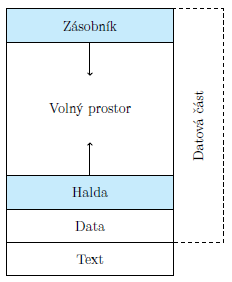
\includegraphics[width=\textwidth]{images/proc_user_context.png}
		\caption{Uživatelský kontext procesu}
		\label{proc_user_context}
 	\end{minipage}
\hspace*{1em}
 	\begin{minipage}[b]{0.47\textwidth}
		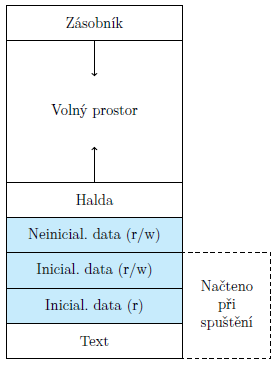
\includegraphics[width=\textwidth]{images/proc_data_segment.png}
		\caption{Datová část paměti procesu}
		\label{proc_data_segment}
	\end{minipage}
\end{figure}

Datový segment lze rozdělit na:

\begin{itemize}
	\item inicializovaná data dostupná pouze pro~čtení -- datové prvky inicializované programem,
	které nelze měnit,
	\item inicializovaná data dostupná pro~čtení i~zápis -- datové prvky inicializované programem,
	ovšem jejich hodnoty mohou být za~běhu procesu měněny,
	\item neinicializovaná data -- datové prvky, které program neinicializoval. Neinicializovaná data lze měnit za~běhu procesu.
\end{itemize}

\subsection{Kontext jádra}

V~tabulce PCB (Řídící tabulka procesů, \emph{Process Control Block}) jsou obsaženy informace o~všech spuštěných procesech. Identifikátor PID funguje jako index procesu.

Jsou zde udržovány informace o~rozložení uživatelského kontextu a~další data k~jeho správě:

\begin{itemize}
	\item Programový čítač -- obsahuje adresu následující instrukce procesu, která bude vykonána procesorem.
	\item Parametry spojené s~plánováním běhu procesů -- priorita procesu, čas aktivity v~CPU, ukazatel na~plánovací frontu atd. Tyto informace jsou použity při~plánování procesů, tj. rozhodování, který proces je na~řadě.
	\item Seznam vstupů a~výstupů využívané procesem -- například se může jednat o~seznam otevřených souborů.
	\item Stav činnosti procesu.
\end{itemize}

\begin{table}[ht]
	\centering
	\begin{tabular}{l|l}
	nový       & připraven k~vytvoření \\
	připravený & proces čeká na~přidělení procesoru \\
	vykonávaný & instrukce jsou prováděny \\
	čekající   & proces čeká na~událost (načtení dat) \\
	ukončený   & proces dokončil vykonávání instrukcí \\
	\end{tabular}
	\caption{Stavy procesu}
\end{table}

Po~vytvoření procesu je ve~stavu \emph{připravený}. Poté, co je vybrán plánovačem procesů, je \emph{vykonáván}. Vykonávání se ukončí buď dobrovolným opuštěním procesu, nebo v~případě příchozího přerušení, nebo zablokování procesu z~důvodu čekání na~určitou událost (načítání dat). Při~zablokování (potom co proces již není ve~stavu čekání) je opět ve~stavu \emph{připravený}. A celý \enquote{cyklus} se opakuje. Když proces svou práci dokončí, přejde do~stavu \emph{ukončený}, do~kterého lze přejít pouze ze~stavu \emph{vykonávaný}! Při~změně vykonávání procesu (přepnutí kontextu) se aktuální stav běhu procesu uloží v~řídící tabulce procesů, ze~které se i~načítá poslední stav běhu procesu.

\begin{figure}
	\centering
	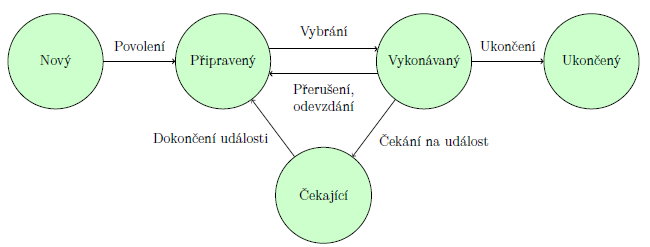
\includegraphics[scale=1]{images/proc_states.png}
	\caption{Přechody mezi stavy procesu}
	\label{proc_states}
\end{figure}

\subsection{Vlákna}

Vlákna si lze představit jako stavební bloky procesů, které jsou jimi vykonávané. Proces může mít jedno či~více vláken. Pokud běží pouze na~jednom, může provádět pouze jeden úkol v~daném čase. S~více vlákny lze pracovat na~více úkolech najednou, případně vykonávat stejný úkol nad~různými daty (webserver). Aby tyto úkoly šlo vykonávat ve~stejném čase, musí být přítomno buď více procesorů, nebo více jader v~procesoru (jedno jádro resp. jeden procesor vykonává jedno vlákno). Každé vlákno má vlastní zásobník, ale sdílí zbytek uživatelského kontextu (tj. datový i~textový segment a~haldu)!

Využitím sdíleného uživatelského kontextu programátor zajišťuje hladký průběh paralelizace: při~sdílení dat mezi vlákny může dojít ke~čtení nekonzistentních dat, tj. k~souběhu (viz otázku~\ref{sync}).

Z~pohledu správy lze vlákna rozdělit na~dva typy: \emph{vlákna jádra} (z~programu jádra) a~\emph{uživatelská vlákna} (z~programů mimo jádro). Mezi uživatelskými vlákny a~vlákny jádra existuje několik možných návazností/modelů:

\begin{figure}[ht]
	\centering
	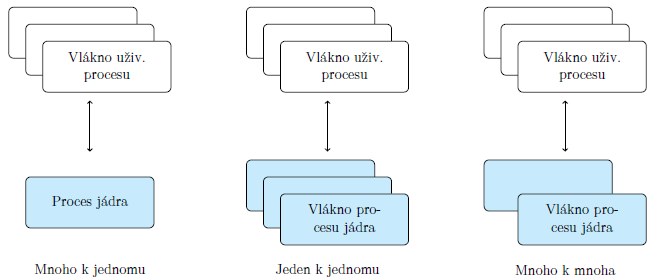
\includegraphics[scale=1]{images/thread_models.png}
	\caption{Vazby procesů a vláken}
	\label{thread_models}
\end{figure}

\begin{itemize}
	\item Mnoho k~jednomu -- Jednomu procesu jádra patří více uživatelských vláken. Použití vláken není závislé na~jejich podpoře v~OS a~jejich správa je zajištěna často v~podobě \emph{vláknových knihoven} (v~uživatelském režimu). Tyto knihovny vytváří a~plánují běh, přepínají a~ruší vlákna. Nevýhodou je fakt, že zavolání blokujícího systémového volání jedním z~vláken zablokuje celý proces (tedy všechna vlákna), jelikož jádro s~vlákny nepracuje.
	\item Jeden k~jednomu -- Každé uživatelské jádro má korespondující vlákno v~jádře a~tedy má i~na~starosti jejich správu. Výhodou je, že blokující systémové volání neblokuje všechna ostatní vlákna. Dále je umožněn běh paralelně na~více procesorech. Nevýhodou je značná režie, skrz vysoké množství vláken.
	\item Mnoho k~mnoha -- Kombinace předešlých, přiřazuje vláknům stejný nebo menší počet vláken v~jádru. Počet těchto vláken může být omezen vzhledem k~aplikaci nebo druhu zařízení (např. jednoprocesorové vs. víceprocesorové).
\end{itemize}

%%%%%%%%%%%%%%%%%%%
% ČINNOST PROCESŮ %
%%%%%%%%%%%%%%%%%%%

\clearpage
\section{Činnost procesů -- stavy činnosti, rozšířený stavový model běhu procesů}
\label{proces-work}

Dříve vyjmenované stavy (obrázek \ref{proc_states} v~otázce \ref{procesy}) nejsou kompletní výčet. Skutečný stavový model má devět položek, kterými jsou:

\begin{enumerate}
	\item Proces je vykonáván v~uživatelském režimu
	\item Proces je vykonáván v~režimu jádra
	\item Proces je připraven ke~zpracování a~je uložen v~hlavní paměti
	\item Proces je spící a~je uložen v~hlavní paměti
	\item Proces je připraven ke~zpracování a~je uložen v~odkládací paměti
	\item Proces je spící a~je uložen v~odkládací paměti
	\item Vykonávání procesu je nuceně přerušeno
	\item Proces je vytvořený a~je v~přechodovém stavu
	\item Proces je ve~stavu \emph{zombie}, neexistuje, ale v~systému je o~něm záznam
\end{enumerate}

\begin{figure}[ht]
	\centering
	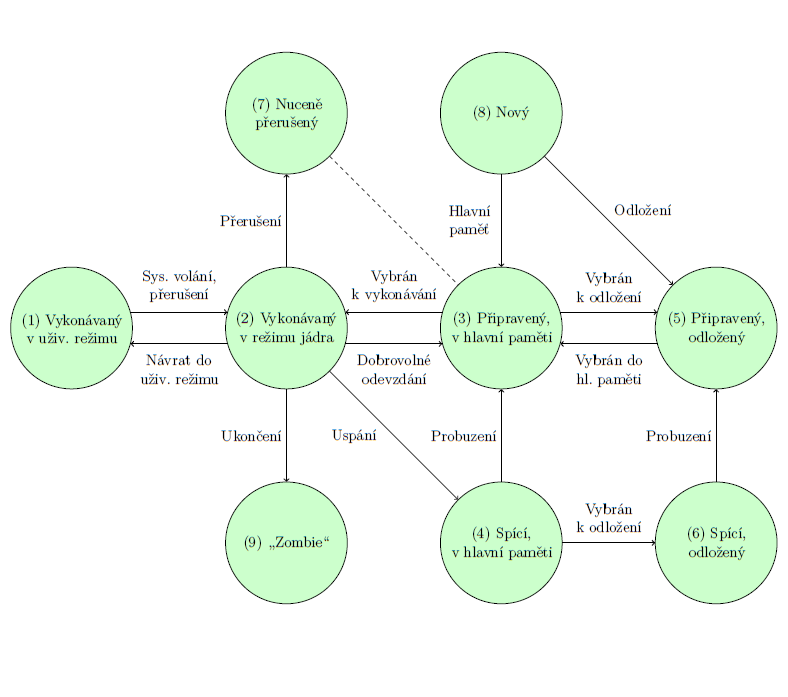
\includegraphics[width=\textwidth]{images/proc_extended_states.png}
	\caption{Rozšířené stavy procesů}
	\label{proc_extended_states}
\end{figure}

Je důležité si všimnout, že se jedná o~rozšíření zkráceného modelu: stav \enquote{vykonávaný} je zde rozšířen o~informaci v~jakém režimu běží. Do~režimu jádra se proces dostane pomocí systémových volání nebo přerušení, jinak (s výjimkou jádru vlastních procesů) běží v~uživatelském režimu.

Stav \enquote{čekající} je zde rozšířen na~\enquote{spící a~uložen v~hlavní paměti} a~\enquote{spící a~uložen v~odkládací paměti}. Přechod mezi těmito dvěma stavy řídí plánovač II. úrovně, který vyměňuje procesy mezi hlavní (RAM) a~odkládací pamětí (swap na~disku). Změna stavu zde může být pouze do~odkládací paměti.

\enquote{Připravený} je nahrazen stavy \enquote{připravený ke~zpracování a~uložen v~hlavní paměti} a~\enquote{připraven ke~zpracování a~uložen v~odkládací paměti}. Přechod je zde opět dán plánovačem II. úrovně. Tentokrát však dochází k~obousměrným přechodům.

\enquote{Proces v~hlavní paměti} zahrnuje stavy \enquote{připraven ke~zpracování a~uložen v~hlavní paměti} a~\enquote{spící a~uložen v~hlavní paměti}. Přechod mezi těmito stavy je jednosměrný a~je způsoben probuzením procesu (dočkáním se na~událost kvůli které byl uspán).

\enquote{Proces v~odkládací paměti} zahrnuje stavy \enquote{připraven ke~zpracování a~uložen v~odkládací paměti} a~\enquote{spící uložen v~odkládací paměti}. Přechod funguje stejně jako v~předešlém odstavci.

\subsection{Více do~hloubky}

\subsubsection{Vytvoření procesu}

Proces vzniká pomocí systémového volání \emph{fork}, kde se z~původního procesu (\emph{rodič}) vytvoří nový proces (\emph{potomek}). Pro~možnost identifikace rodiče potomka se zavádí identifikátor \emph{PPID} (Parent Process IDentifier); zároveň zpravidla platí, že proces má jednoho rodiče, ale rodič může mít více potomků%
\footnote{Všechny procesy jsou následovníkem procesu \emph{init}.}%
.

Systémové volání \emph{fork} je voláno rodičem jednou, ale vrací se dvakrát: do~procesu rodiče (s~PID nového procesu) a~do~procesu potomka (s~PID $= 0$). To zjednodušuje rozlišení potomka a~rodiče při~programování; potomek následně volá systémové volání \emph{execve}, kterým spustí programový kód nového procesu. \emph{Fork} vytvoří kopii rodičovského procesu, existují pak tedy dva stejné procesy.

\emph{Fork} je vykonáván v~režimu jádra. Vyhledá se volná pozice v~tabulce procesů a~obsadí se záznamem potomka (jeho kontext jádra, viz otázku \ref{procesy}) a~poté se alokuje paměť pro~uživatelský kontext potomka (taktéž v~kapitole \ref{procesy}), který se naplní kopií uživatelského kontextu rodiče%
\footnote{Textová část může být buď kopírována nebo sdílena.}%
. Proces skončí jakmile dokončí svůj kód a~vyvolá systémové volání pro~své ukončení (např. \emph{exit}). Proces však nemusí ukončit jen sám sebe; pokud má dostatečná oprávnění, může ukončit i~jiný proces. Po~ukončení procesu je rodiči navrácen PID ukončeného procesu.

Proces může ze~stavu \enquote{vytvořený} přejít do~stavu \enquote{připraven na~zpracování}, záleží však kolik je volného místa v~paměti. Pokud je ho dost, tak přejde do~stavu \enquote{připraven ke~zpracování v~hlavní paměti}, kde čeká až jej vybere plánovač I. úrovně a~pak přejde do~stavu \enquote{vykonávaný v~režimu jádra}, kde se obslouží systémové volání. Nakonec přejde do~režimu \enquote{vykonáván v~uživatelském režimu}.

\subsubsection{Vykonávání procesu}

Proces je vykonáván buď v~režimu jádra nebo v~uživatelském režimu, kde přechází do~režimu jádra pomocí volání systémového volání a~obsluhy přerušení. Procesy se nestřídají pouze po~dokončení práce nebo při~dobrovolném čekání. Může totiž docházet i~k preemptivnímu střídání procesů, kdy každý proces má povolenou maximální dobu vykonávání. Pokud tato doba uběhne, je proces přerušen a~přejde do~stavu \enquote{nuceně přerušený} (který je totožný se stavem \enquote{připraven na~zpracování v~hlavní paměti}%
\footnote{Jediný rozdíl je v~tom jak se proces do~tohoto stavu dostal.}%
). Plánovač pak vybere jiný proces k~vykonávání.

Druhou možností je, že proces se dobrovolně ukončí před uplynutím maximálního časového intervalu a~opět přejde do~stavu \enquote{připraven ke~zpracování v~hlavní paměti}.

\subsubsection{Uspání procesu}

Předpokládejme proces čekající na IO (vstupně-výstupní) operaci. Zavolá systémové volání pro~zápis/čtení dat a~přejde ze~stavu \enquote{vykonáván v~uživatelském režimu} do~stavu \enquote{vykonáván v~režimu jádra}. Aby proces neplýtval zdroje čekáním v~tomto stavu, sám se zablokuje (\enquote{uspí}) a~přejde do~stavu \enquote{spící v~hlavní paměti}. Tímto uvolní místo pro~jiný proces čekající v~hlavní paměti.

Po~dokončení operace je proces probuzen a~je připraven v~hlavní paměti. Zde čeká až jej vybere plánovač I. úrovně.

\subsubsection{Odložení procesu}

Pokud je v~systému spuštěno tolik procesů, že se nevejdou do~hlavní paměti přichází na~řadu plánovač II. úrovně (tzv. vyměňovací proces), který vybírá procesy k~přesunutí z~hlavní paměti do~paměti odkládací (\enquote{připravený v~hlavní paměti} $\rightarrow$ \enquote{připravený, odložený}). Stejně tak může přesouvat spící procesy z~hlavní paměti do~odkládací paměti. Po~probuzení jej může plánovač opět přesunout zpět do~hlavní paměti.

Je třeba mít na~vědomí, že plánovač II. úrovně vybírá procesy tak aby se všechny vystřídaly v~hlavní paměti. Tam pak čekají na~plánovač I. úrovně.

\subsubsection{Ukončení procesu}

Proces v~uživatelském režimu zavolá sys. volání (např. dříve zmíněný \emph{exit}), přejde tedy do~režimu jádra a~dále do~stavu \enquote{zombie}. V~tomto stavu proces neexistuje, ale je o~něm stále udržován záznam v~tabulce procesů. Jakmile rodič zpracuje informaci o~jeho ukončení, tak je proces definitivně ukončen.

%%%%%%%%%%%%%%
% SCHEDULING %
%%%%%%%%%%%%%%

\clearpage
\section{Plánování procesů -- okamžiky rozhodnutí, plánovací algoritmy, systém priorit}
\label{planning}

V~dnešní době se plánování procesů (\emph{scheduling}) provádí na~více procesorech a~jádrech. Aby každý proces přišel na~řadu a nebyl vynechán, využívá se plánovač (\emph{process scheduler}) a~plánovací algoritmy. Využívají se za~účelem navození pocitu, že vše v~Operačním Systému běží současně, přitom se jedná o~neustálé a~rychlé přepínání kontextu.

\subsection{Okamžiky rozhodnutí}

Okamžiky, kdy se plánovač musí rozhodnout který proces bude vykonáván jsou následující: \emph{vytvoření procesu} (bude se vykonávat rodič, potome, nebo jiný proces?), \emph{ukončení}, \emph{blokování} a~\emph{přerušení} od~zařízení nebo hodin (bude se vykonávat jaký proces?).

Průběh při~výkonu dvou procesů lze jednoduše ukázat na~obrázku \ref{proc_changing}. Procesy se střídají podle toho, který zrovna čeká (např. na~I/O operaci). Při~takovém přerušení může dojít k~rozhodnutí o~přepnutí procesu. Toto přepnutí může být provedeno při~každém \emph{n}-tém přerušení.

Je také třeba rozlišovat nepreemptivní (kooperativní) a~preemptivní systémy. V~prvním případě dochází k~přepínání pouze pokud proces dobrovolně uvolní procesor. Ve~druhém případě se přepíná na~základě nuceného přerušení od~hodin, kdy pak plánovač zvolí jiný proces k~vykonávání.

\begin{figure}[ht]
	\centering
	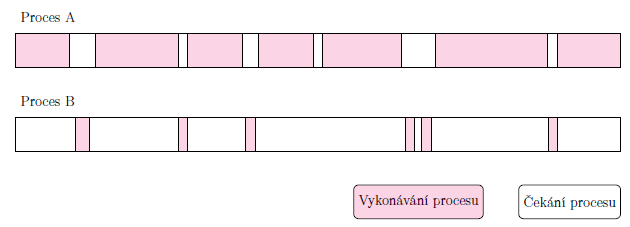
\includegraphics[scale=1]{images/proc_changing.png}
	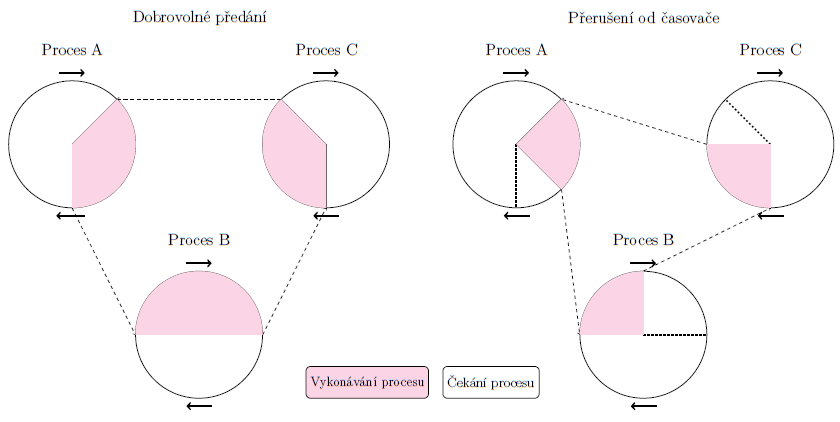
\includegraphics[scale=1]{images/proc_preemption.png}
	\caption{Sdílení procesoru více vlákny}
	\label{proc_changing}
\end{figure}

\subsection{Typy plánovacích algoritmů}

Ne všechny počítače mají stejný účel, např. letové systémy vyžadují co nejrychlejší odezvu v~určeném časovém úseku na~rozdíl od~našeho domácího počítače, který upředostňuje komfort a~ne splňování \emph{deadlinů}.

\subsubsection{Dávkové systémy}

\emph{Batch} systémy zpracovávají úkoly v~tzv. dávkách bez účasti uživatele. Tímto jsou eliminovány prodlevy způsobené čekáním na~akce od~uživatele. Používá se nepreemptivních plánovačů (tedy proces sám musí uvolnit procesor).

Příklady jsou systémy od~IBM a~GCOS (General Comprehensive Operating System) od~firmy Bull SAS.

Tyto systémy jsou typické pro~nákladná a~výkonná informační centra, kde je prioritou co nejlépe využít drahý hardware. Sledují se především tyto parametry:

\begin{itemize}
	\item Výkonnost -- počet úloh zpracovaných za~jednotku času%
	\footnote{Plánovač zvyšující výkonnost nemusí nutně zvyšovat rychlost obsluhy. Za~účelem zvýšení výkonnosti může upřednostňovat kratší úlohy, na~které se však musí déle čekat. Výkonnost stoupá, ale rychlost obsluhy klesá.}%
	.
	\item Rychlost obsluhy -- průměrný čas od~doby přijetí požadavku do~jeho splnění.
	\item Využití CPU -- preferuje se maximální využití a~minimální prostoje.
\end{itemize}

\subsubsection{Interaktivní systémy}

Chod systému je ovlivňován uživatelem a~jeho požadavky by měly být vyřizovány přednostně. Uživatel předpokládá, že program který má právě v~popředí bude pracovat co nejrychleji a~stejně tak reagovat, interaktivní systémy se snaží tento předpoklad splnit. Plánovač sice nemůže ovlivnit složitost úlohy a~rychlost zpracování, může však přispět ke~splnění očekávání uživatele. Je zřejmé, že se upřednostňuje užívání preemptivního přepínání, aby nemohl žádný proces zabrat CPU na~příliš dlouhou dobu.

Sleduje se čas odezvy (od~vyslání příkazu po~obdržení výsledku) a~přeiměřenost (složitost úlohy k~době jejího zpracování).

Jedná se o~klasické desktop systémy jako Windows, MacOS a~různé distribuce OS Linux.

\subsubsection{Real-Time systémy}

Používají se pro~zpracování úloh které slouží jako vstup dalších navazujících činností. Tyto systémy musí splnit úlohu v~reálném čase (v~předem daném časovém úseku). Tyto systémy jsou používány v~automatizovaných procesech, robotice a~telekomunikacích. Používá se opět preemptivní plánování.

Podle toho jak moc se tlačí na~splnění požadavků v~daném času můžeme tyto systémy dělit na~\emph{soft} (časové zárky jsou pouze přibližné a~určité časové odchylky jsou povoleny) a~\emph{hard} (časové záruky jsou plně zajištěny).

Jsou sledovány parametry jako dodržování časových termínů (což je nejdůležitější požadavek) a~předvídatelnost a~pravidelnost (např. systémy se zpracováním multimediálních dat).

Příkladem real-time systémů jsou \href{https://github.com/FreeRTOS/FreeRTOS}{FreeRTOS} nebo~VxWorks od~firmy Wind River.

Na~základě znalosti času potřebného k~obsloužení periodických událostí můžeme prohlásit, zda je systém schopný činnosti. Mějme $m$ periodických událostí, kde se událost $i$ vyskytuje s~periodou $\mathrm{P}_i$ a~vyžaduje $\mathrm{C}_i$ procesorového času. Aby byl real-systém běhuschopný, musí splňovat podmínku
$$\sum\limits_{i=1}^m \frac{C_i}{P_i} \leq 1.$$

\subsection{Systém priorit}

Plánovač I. úrovně vybírá procesy, které jsou připravené v~hlavní paměti, aby získaly procesorový čas. Algoritmus plánování je postaven na~\emph{paralelních frontách}, kde je každá fronta spojena s~intervalem priorit. Uživatelské procesy mají kladnou prioritu a~procesy jádra mají záporné hodnoty%
\footnote{Kladné hodnoty uživatelských procesů a~záporné procesů jádra platí pro~UNIX a~Linux.}%
. Z~toho vyplývá, že nižší hodnota znamená vyšší prioritu (tj. procesy jádra mají nejvyšší prioritu, protože obsluhují systémová volání).

Plánovač prochází fronty od~nejnižších intervalů (nejvyšší priorita) dokud nenalezne obsazenou frontu. Poté vybere první proces z~dané fronty a~po vykonání je vložen na~konec místní fronty (\emph{round-robin}). Priorita každého procesu je počítána (pro začátek každého intervalu, např. každou sekundu) pomocí vzorce $P = V + N + B$.

Podle této nové priority je proces přiřazen do~fronty. Fronta bývá zvolena na~základě dělení vypočtené priority zvolenou konstantou.

$V$ je čítač představující využití procesoru. Tato hodnota se inkrementuje s~každým taktem procesorových hodin (pokud je proces vykonáván na~procesoru). Tímto způsobem se upřednostňují nové procesy, které ještě nezískaly procesorový čas. Zároveň lze procesy co zrovna využily procesor penalizovat pomocí navýšení původní hodnoty $V$ o~aktuální hodnotu z~daného intervalu a~výsledek je vydělen dvěma. Tímto způsobem jsou penalizovány nedávno vykonané procesy a~předchází se \emph{stárnutí procesů}.

Hodnota $N$ (tj. \emph{nice}) je implicitně nastavena na~0 (povolený rozsah je -20 až +19) a~je zděděna od~rodičovského procesu. Běžný uživatel může nastavovat hodnoty $0$ -- $19$ a~tím penalizovat vlastní procesy, administrátor může procesy preferovat snížením hodnoty nice na~$-20$ -- $-1$.

$B$ (\emph{báze}) je použita pokud se proces zablokuje (např. protože čeká na~I/O operaci). Je odstraněn z~plánovací fronty (jelikož není ve~stavu \emph{připraven}). Je znovu zařazen do~fronty po~přijetí události, ale s~jinou prioritou. Volba fronty/priority závisí na~události, na~kterou proces čekal (nastaví se hodnota $B$).

%%%%%%%%%%%%%%%%%
% SYNCHRONIZACE %
%%%%%%%%%%%%%%%%%
\clearpage
\section{Synchronizace procesů -- souběh, vzájemné vyloučení, uvíznutí procesů}
\label{sync}

Zajištění synchronizace je zásadní problém v~jakémkoliv paralelně běžícím systému. Jeden proces může svým během ovlivnit jiný proces nebo jím být ovlivněn, a~aby k~tomu nedošlo zavádíme synchronizační techniky: vyloučení konfliktu kritických činností pro~zamezení souběhu a~zajištění časové souslednosti pro~paralelní programování.

\subsection{Souběh}

Souběh nastává při~práci procesů se sdílenými prostředky. Fronta tiskárny s~ukazatelem \emph{in} ukazuje poslední volné místo ve~frontě. Proces A načte z~fronty informaci že první volné místo je na~pozici 10 a~tuto informaci uloží do~lokální proměnné. Následně však plánovač přepne kontext na~proces B, který udělá to stejné a~uloží svůj soubor na~index 10 a~inkrementuje jej na~11. Plánovač poté přepne kontext zpět na~proces A, který má stále uloženou hodnotu 10, čímž soubor procesu B přepíše.

\begin{figure}[ht]
	\centering
	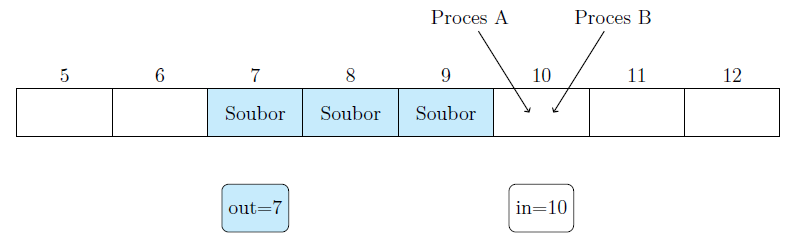
\includegraphics[width=\textwidth]{images/proc_soubeh.png}
	\caption{Souběh procesů}
	\label{proc_soubeh}
\end{figure}

Toto čtení nekonzistentních dat z~důvodu přepnutí kontextu nazýváme \emph{souběh} tj. \emph{race condition}. Problémem je, že k~souběhu nemusí vždy dojít a~záleží čistě na~plánovači a~kdy dojde k~přepnutí kontextu, proto se tato chyba velmi špatně zachytává při~testování.

\subsubsection{Zajištění časové souslednosti}

Proces musí čekat na~dokončení celé množiny operací, než může pokračovat. Toho lze docílit pomocí paralelního programování za~využití vláken a~tzv. \emph{bariér}/\emph{časových mezníků}.

Představme si aplikaci používající vlákna. Všechny vlákna musí dokončit svou úlohu z~fáze 1 než mohou přejít do~fáze 2 a~i když vlákna vykonávají stejný kód, tak mohou pracovat různými rychlostmi. Pokud nějaké vlákno skončí s~úlohou z~fáze 1 dřív jak jiné, bude pozastaveno než je dokončí všechny ostatní vlákna.

\begin{figure}[ht]
	\centering
	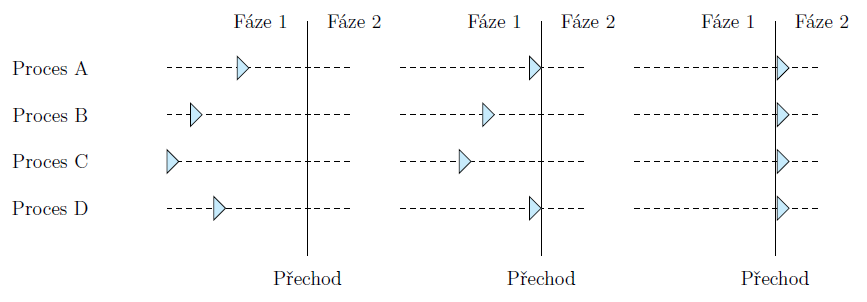
\includegraphics[width=\textwidth]{images/proc_barrier.png}
	\caption{Bariéra}
	\label{proc_barrier}
\end{figure}

\subsubsection{Vzájemné vyloučení pomocí kritické sekce}

Souběhu lze zabránit výlučným přístupem ke~sdílenému prostředku, tedy že dokud jeden proces pracuje se sdíleným prostředkem, ostatní jsou zablokované a~čekají na~uvolnění prostředku. Tohoto lze docílit například pomocí určení části kódu, kterou označíme za~\emph{kritickou sekci}, ve~které se smí nacházet vždy nanejvýše jeden proces.

Této myšlence se obecně říká \emph{zámek} (tj. \emph{mutex}): přístup ke~sdílené proměnné je uzamčen pro~ostatní procesy. Mezi často používané patří například semafory. Proces zkontroluje zámek, a~pokud je \emph{odemčený}, \emph{zamkne} jej a~přistoupí k~proměnné (vstoupí do~kritické sekce). Po~dokončení operací zámek \emph{odemkne} a~umožní přístup ostatním procesům.

Krom vzájemné vyloučení je potřeba zajistit i~následující podmínky:

\begin{enumerate}
	\item Blokování jiného procesu je pouze možné v~případě, že jiný proces je v~kritické sekci. Blokování procesem mimo KS je nepřijatelné.
	\item Doba čekání na~vstup do~kritické sekce musí být konečná.
\end{enumerate}

\subsubsection{Vzájemné vyloučení pomocí proměnných}

% TODO Co to tu přesně znamená? Nebylo by lepší to napsat větou?
\begin{itemize}
	\item Sdílená dvouhodnotová proměnná
	\item Striktní střídání procesů
\end{itemize}

\paragraph{Sdílená dvouhodnotová proměnná}

Mějme sdílenou proměnnou \emph{lock}, která může nabývat stavů \emph{FALSE} a~\emph{TRUE}. \emph{FALSE} značí, že v~kritické sekci není žádný proces a~\emph{TRUE} značí obsazenou kritickou sekci. Proces tedy před vstupem do~KS zkontroluje proměnnou a~postupuje tak jak bylo popsáno dříve. Pokud je \emph{lock} uzamčený (\emph{TRUE}), proces čeká v~čekající smyčce%
\footnote{Čekání ve~smyčce na~odemknutí zámku se nazývá aktivní čekání a~jedná se o~skvělý způsob jak plýtvat zdroji.}
na~uvolnění prostředků.

Tento způsob je náchylný na~souběh. Může se stát, že proces A přistoupí k~zámku a~načte jeho hodnotu jako \emph{FALSE}, poté plánovač přepne kontext na~proces B, který vstoupí do~kritické sekce, a~nastaví \emph{lock} na~\emph{TRUE}. Plánovač opět přepne kontext a~proces A vstoupí do~kritické sekce, výsledkem jsou dva procesy v~kritické sekci najednou.

\paragraph{Striktní střídání procesů}

Opět může být docíleno pomocí sdílené dvoustavové proměnné, např. \emph{turn} nabývající hodnot 0 a~1 (0 = A, 1 = B). Pokud obsahuje hodnotu 0, tak proces A může vstoupit do~KS a~proces B je v~čekací smyčce. Po~dokončení práce procesu A, je \emph{turn} nastaven na~1.

Problém nastává když jeden z~procesů vstupuje do~KS častěji jak druhý. Pak je například hodnota \emph{turn} nastavena na~1 a~proces A musí čekat na~proces B, který však zatím ani v~KS není. Tímto se porušilo pravidlo, že proces může být blokován pouze procesem v~kritické sekci.

\subsubsection{Vzájemné vyloučení pomocí hardwarových funkcí}

\paragraph{Zákaz přerušení}

Toto řešení platí pro~preemptivní systémy, kde se zákazem přerušení na~procesoru zajistí tím, že proces nelze přerušit dokud nevystoupí z~kritické sekce. Přerušení mohou obecně zakazovat uživatelské i~systémové programy, ovšem povolit zakazování přerušení pro~uživatelský program je velmi riskantní.

Tento přístup však funguje pouze na~jednoprocesorových systémech. Pokud je procesorů více, tak na~jednom je přerušení sice zakázáno, ale tento zákaz neplatí pro~procesy na~ostatních procesorech. Zavedení zákazu přerušení na~všech procesorech by vyžadovalo zaslání zprávy všem procesorům, což je časově neefektivní operace.

\paragraph{Atomické funkce}

Jedná se o~instrukce, které umožní číst a~měnit hodnotu (nebo zaměnit obsah dvou proměnných) a~nelze je přerušit. Princip lze pochopit na~instrukci \emph{TestAndSet} (tj. \emph{TSL -- Test and Set Lock}). Tato instrukce testuje proměnnou, pokud je nastavena na~FALSE nastaví na~TRUE a~proces vstoupí do~KS. Ostatní procesy potom čekají v~aktivní smyčce (opakovaně volají \emph{TestAndSet} dokud není \emph{lock} opět FALSE). Poté co proces skončí v~KS nastaví proměnnou na~FALSE.

Princip je podobný jako u~přístupu se sdílenou proměnnou, krom toho že instrukce je nepřerušitelná, tedy nemůže dojít k~přepnutí kontextu a~tím pádem k~souběhu.

\subsubsection{Vzájemné vyloučení pomocí systémového volání}

Předešlé metody využívají aktivního čekání, které má následující nevýhody:

\begin{itemize}
	\item Plýtvání časem CPU%
	\footnote{Za~předpokladu, že se nebude čekat moc dlouho, jde využít aktivního čekání.}.
	\item Porušení základní podmínky, že čekání na~vstup do~kritické sekce musí být konečná.
\end{itemize}

Další problém se kterým se můžeme u~paralelizmu setkat, je \emph{problém opačné priority}. Pokud máme dva procesy, kde proces A má vyšší prioritu jak B a~proces B je v~kritické sekci. Plánovač zvolí k~vykonání proces A (s vyšší prioritou), který čeká na~přístup do~KS. Jelikož je však procesu A dávána přednost, tak proces B nikdy z~KS nevystoupí.

Procesy se mohou navzájem uspávat, v~tomto případě by tedy proces A uspal B a~zaslal by mu signál na~probuzení až po~výstupu z~KS. I~zde však může nastat souběh. Toto lze ilustrovat na~tzv. \emph{producer-consumer problem}, kde máme dva procesy, jednoho producenta a~spotřebitele. Procesy pracují se sdílenou pamětí o~omezené velikosti, producent paměť naplňuje a~jakmile je plná tak přejde do~režimu spánku, následně spotřebitel odebere položku z~paměti, čímž probudí producenta. Pokud chce spotřebitel odebrat z~paměti a~je prázdná tak se uspí. Ke sledování stavu v~paměti se může použít sdílené proměnné (\emph{counter}) a~komunikace probíhá pomocí sys. volání.

Pokud je paměť prázdná ($counter = 0$), spotřebitel přečte hodnotu sdílené proměnné, ale před uspáním dojde k~přepnutí kontextu. Producent uvidí, že paměť je prázdná a~začne ji naplňovat. Jakmile zvýší proměnnou o~jedna, zavolá systémové volání aby probudil spotřebitele (v domnění že je uspaný), a~tím že spotřebitel nespí nemá volání žádný účinek. Producent tedy kompletně naplní paměť a~uspí se. Dojde k~přepnutí kontextu a~spotřebitel se také uspí. Došlo tedy k~\emph{fatálnímu souběhu}.

\subsection{Uvíznutí, tj. Deadlock}

Skupina procesů je ve~stavu uvíznutí, pokud každý z~nich čeká na~událost, kterou může způsobit pouze jiný proces z~této skupiny. Uvíznutí může nastat nad různými prostředky (hardwarové či softwarové), které dělíme na~\emph{sdílitelné} (globální proměnné, sdílený úsek paměti, záznam v~databázi, ...) a~\emph{nesdílitelné} (tiskárny, scannery, DVD, ...). Sdílené prostředky mohou být uzamčené. Dále lze rozdělit na~\emph{přepínatelné}%
\footnote{Uvíznutí nenastává nad sdílitelnými prostředky bez jejich uzamčení, nebo nad přepínatelnými prostředky kde lze uvíznutí předejít předáním jinému procesu.} %
a~\emph{nepřepínatelné}%
\footnote{Odebrání přepínatelného prostředku nezpůsobí žádnou škodu -- např. hlavní paměť. Nepřepínatelný prostředek je takový, jehož odebrání způsobí nefunkčnost procesu.}%
.

Využití sdíleného prostředku se skládá ze~tří částí:

\begin{enumerate}
	\item Žádost -- Proces žádá o~využití prostředku a~aktivně čeká pokud je využitý
	\item Používání -- Proces využívá prostředek
	\item Uvolnění -- Proces ukončil práci a~předal o~tom zprávu
\end{enumerate}

Důvody k~uvíznutí mohou být například stav, kdy první proces čeká na~prostředek obsazený druhým procesem, který je také ve~stavu čekání na~prostředek obsazený prvním procesem (obrázek \ref{proc_deadlock}). Často se jedná i~o chybu v~programu při~předávání informace o~využívání prostředku.

\begin{figure}[ht]
	\centering
	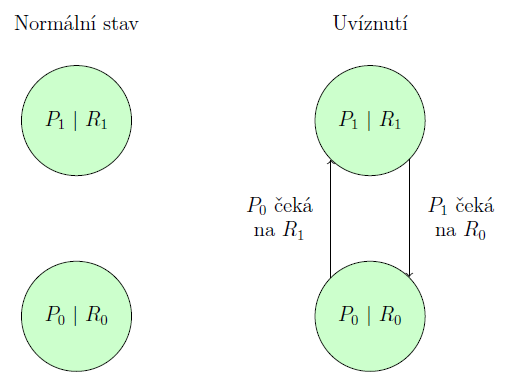
\includegraphics[scale=0.5]{images/proc_deadlock.png}
	\caption{Deadlock}
	\label{proc_deadlock}
\end{figure}

Tato situace lze řešít předcházením uvíznutí, připuštěním že se systém do~stavu uvíznutí dostat může, umí tento stav detekovat a~obnovit činnost, nebo ignorováním tohoto problému. Detekce a~napravení deadlocku vyžaduje neustálé spouštění algoritmu se dvěma metodami obnovení činnosti:

\begin{itemize}
	\item Procesy ve~stavu uvíznutí jsou násilně ukončeny:
	\begin{enumerate}
		\item postupně -- pomalejší řešení, po~každém ukončeném procesu je potřeba znovu spustit detekční algoritmus, volba procesu může být například na~základě stáří
		\item všechny najednou -- rychlejší řešení s~velkými náklady (například ztráta předešlých výpočtů a~dat)
	\end{enumerate}
	
	\item Procesům jsou násilně odebrány všechny prostředky a~předávány jiným procesům ve~stavu uvíznutí. Po~každém odebrání je opět potřeba spustit detekční algoritmus, aby se zjistilo zda bylo uvíznutí vyřešeno.
\end{itemize}

%%%%%%%%%%%%%%%%%
% SPRÁVA PAMĚTI~%
%%%%%%%%%%%%%%%%%

\clearpage
\section{Správa paměti -- vyměňování procesů, virtuální paměť pomocí stránkování a~segmentace}

Paměť dělíme na~dvě části:
\begin{itemize}
	\item Fyzický Adresový Prostor (FAP; hlavní paměť, RAM) -- reálná kapacita fyzické paměti v~počítači která je dána nainstalovanou pamětí. Aby proces byl vykonáván musí být celý, nebo jeho vykonávaná část, v~RAM paměti. Hlavní důvod je rychlost přístupu do~této paměti.
	\item Logický Adresový Prosto (LAP; vedlejší paměť, virtuální paměť) -- jedná se o~paměť tak jak ji vidí procesy. Určená adresami, které je proces/OS schopen generovat. LAP zahrnuje jak FAP (tedy RAM paměť), tak \emph{odkládací prostor}.
\end{itemize}

\begin{figure}[ht]
	\centering
	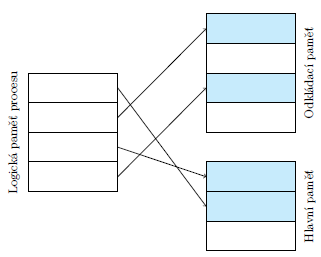
\includegraphics[scale=1]{images/mem_lap.png}
	\caption{Logický adresový prostor}
	\label{mem_lap}
\end{figure}

Pokud počítač pracuje s~32bitovými adresami, může nabízet 4 GiB ($2^{32}$) LAP, i~když má fyzicky pouze 256 MiB FAP. Virtuální paměť lze realizovat vyměňováním procesů, stránkováním nebo segmentací.

\subsection{Vyměňování procesů}

Paměť lze přidělovat celým procesům nebo jejich částem. Ty jsou poté vyměňovány mezi hlavní a~odkládací pamětí, tak aby se postupně vyměnily všechny procesy. Při~práci s~celými procesy se načte celý proces do~paměti a~po nějaké době je odložen do~stavu \enquote{připraven v~odkládací paměti}. Po~určité době je vybrán plánovačem II. úrovně k~přesunutí do~hlavní paměti kde bude opět vybrán plánovačem I. úrovně k~vykonání.

Velikost a~umístění využitých paměťových úseků se dynamicky mění podle procesu načteného do~paměti (jaká je aktuální velikost jejich paměťového prostoru). Toto však způsobuje tzv. \emph{externí fragmentaci paměti}, kdy v~paměti vznikají volné úseky, které však nejsou dostatečné velké pro~kterýkoliv proces (nedochází pak k~efektivnímu využívání paměti, viz obrázek \ref{mem_fragmentace}). Tento jev lze sice napravit tzv. \emph{defragmentací}, tedy spojením volných paměťových úseků a~vytvoření souvislého paměťového prostoru.

Aby se mohl tento úsek vytvořit je třeba přesunout všechny procesy do~jednoho souvislého bloku zabrané paměti. Tento proces je časově náročný (navíc by se musel dělat periodicky), proto se k~němu většinou nepřikračuje.

\begin{figure}[ht]
	\centering
	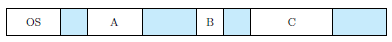
\includegraphics[scale=1]{images/mem_fragmentace.png}
	\caption{Externí fragmentace paměti}
	\label{mem_fragmentace}
\end{figure}

Proces ale lze rozdělit mezi hlavní a~odkládací paměť díky jeho rozdělení na~dílčí části (\emph{overlays}). Lze ho vykonávat pokud má v~paměti svou první část, po~dokončení se načte druhá apod. Nebo je možné držet v~paměti více částí procesu najednou. (viz obrázek \ref{mem_lap}).

\subsection{Stránkování}

Paměťový prostor procesu je rozdělen na~stejně velké části, tzv. \emph{stránky} (\emph{pages}), které jsou v~případě potřeby přesouvány z~odkládací paměti do~stejně velkých míst v~hlavní paměti tzv. \emph{rámců} (\emph{frames}). Přenesení stránek do~hlavní paměti je zavolání tzv. \emph{page fault} (\emph{výpadek stránky}), tedy že proces potřebuje pracovat se stránkou která právě v~paměti není. Proces sám však \emph{page fault} nevyvolá, procesor rozpozná, že chybí stránka a~zavolá \emph{výpadek}\footnote{Proces tuto výměnu ani nevidí, viditelný je pro~OS, který vede evidenci jednotlivých stránek.}. Umístění stránek je uloženo v~\emph{tabulce stránek} (page table).

\begin{center}
	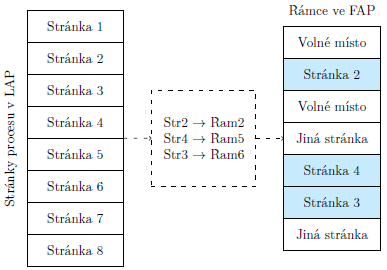
\includegraphics[scale=1]{images/mem_page_table.png}
\end{center}

Díky pevné velikosti stránek je lze efektivně umístit do~stejně velkých rámců. Díky tomu nedochází k~\emph{externí fragmentaci} volného prostoru v~hlavní paměti. Nevýhodou je, že proces do~této struktury nevidí, tudíž neví, že části které patří k~sobě by se měly přesouvat do~paměti společně za~účelem zredukování množství \emph{page fault}.

Důležitým parametrem je volba velikosti stránky, jelikož se stránkováním nemůže docházet k~externí fragmentaci, ale k~interní ano. Pokud jsou stránky moc velké, poslední stránka nebude nikdy kompletně naplněna a~zůstane v~ní nevyužitý prostor. Zároveň pokud proces vyžaduje 4 KiB paměti, ale stránky jsou 32 KiB, je potřeba do~paměti načíst zbytečně 32 KiB. Zřejmě je asi výhodnější mít menší stránky. Na~druhou stranu to však znamená větší počet výpadků stránek a~větší tabulku stránek%
\footnote{Čas přenesení stránky je tvořen převážně jejím vyhledáním, proto doba přenosu malých stránek trvá přibližně stejně jako velkých.}%
.

\subsection{Segmentace}

Pomocí segmentace je paměťový prostor procesů dělen na~logicky související části různé velikosti nazývané \emph{segmenty}. Každý segment má svůj název a~velikost, které vytváří kompilátor podle zdrojového kódu programu. Obecné segmenty mohou být:

\begin{itemize}
	\item Textový -- instrukce programu.
	\item Datový -- inicializované globální a~statické proměnné.
	\item BSS (Block Started by Symbol) -- neinicializované globální a~statické proměnné, kde hodnota může být náhodná hodnota z~paměti nebo O (pro ukazatele \emph{null}).
	\item Halda -- dynamické proměnné.
	\item Zásobník
\end{itemize}

Blíže mohou být segmenty děleny například na~kódy jednotlivých funkcí, velké datové struktury, knihovny linkované s~programem nebo objekty.

Na~rozdíl od~stránkování je segmentace mechanismus, který je procesu viditelný. Pokud proces potřebuje nějakou část segmentu v~hlavní paměti, tak je přenesen celý segment. Výhoda tohoto přístupu je, že jakmile je v~dalších krocích potřeba další část segmentu, nemusí být opět načten do~paměti. Tímto je redukován počet výpadků segmentů (\emph{segment fault}) oproti výpadkům stránek. A stejně tak jako se stránkami vede operační systém záznamy o~všech segmentech v~tabulce segmentů (\emph{segment table}).

\begin{figure}[ht]
	\centering
	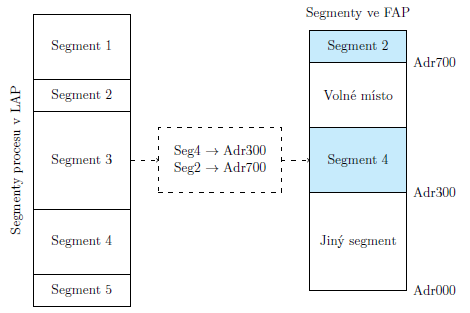
\includegraphics[scale=1]{images/mem_segment_table.png}
	\caption{Segmentační tabulka}
	\label{mem_segment_table}
\end{figure}

Nevýhodou oproti stránkování je dynamická velikost segmentů, což způsobuje externí fragmentaci paměti.

%%%%%%%%%%%%%%%%%%
% VYUŽITÍ PAMĚTI %
%%%%%%%%%%%%%%%%%%

\clearpage
\section{Využití paměti -- přidělování paměti procesům, algoritmy přesunu stránek do~odkládacího prostoru}

Existují tři základní způsoby přidělování hlavní paměti:
\begin{itemize}
	\item rovnoměrně -- nerespektuje rozdílné paměťové nároky procesů a~ani jejich prioritu
	\item podle velikosti procesu -- nerespektuje prioritu procesu
	\item podle velikosti a~priority procesu
\end{itemize}

Aby bylo možné určit počet rámců pro~proces, využívá se metoda na~vyhodnocování frekvence výpadků stránek. Účelem je vyhnout se stavu, kdy je proces zdržován velkým množstvím výpadků stránek, tzv. \emph{trashing}. Ideálním stavem je držení frekvence na~přibližně stejné úrovni; mnoho výpadků značí nedostatek rámců a~málo příliš mnoho paměti. Jedná se o~algoritmus \emph{Page Fault Frequency Replacement}.

\begin{figure}[ht]
	\centering
	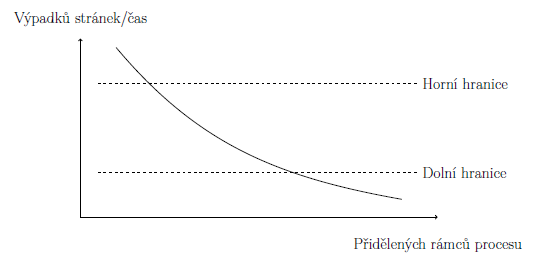
\includegraphics[scale=1]{images/mem_freq_page.png}
	\caption{Graf využití paměti}
	\label{mem_freq_page}
\end{figure}

\subsection{Přesuny stránek}

Virtuální paměť je založena na~odkládání stránek z~hlavní paměti do~odkládací (na~disk). Když je zavolán výpadek stránky je třeba přesunout jednu stránku do~volného rámce. Operační systém zajišťuje že jsou volné rámce vždy dostupné, proto periodicky přesunuje určitý počet stránek do~odkládací paměti.

\subsection{Odkládací paměť}

Při~odložení z~hlavní paměti mohou nastat dvě situace podle dat ve~stránce:

\begin{enumerate}
	\item Data jsou pouze pro~čtení/nebyly provedeny změny -- stránka je z~hlavní paměti smazána
	\item Data byla změněna -- stránka musí být přesunuta do~virtuální paměti
\end{enumerate}

Stránky mohou být svázány s~určitým souborem v~sytému, takový soubor může obsahovat kód procesu (read-only data) nebo se jedná o~soubor připojený do~uživatelského kontextu procesu, tzv. \emph{paměťově mapovaný soubor}%
\footnote{Tyto soubory v~paměti mohou být jak v~režimu pouze pro~čtení tak i~pro~zápis.}%
. Takto lze jednoduše sdílet soubor mezi procesy. Pro~práci s~tímto souborem se používají paměťové funkce, což zvyšuje rychlost operací čtení a~zápisu. Nevýhodou může potencionální plýtvání paměti%
\footnote{Uvažujme stránky o~velikosti 4KiB a~soubor o~velikosti 6KiB, pak musíme využít dvě stránky ale z~toho jsou 2KiB nevyužity.}%
.

\begin{figure}[ht]
	\centering
	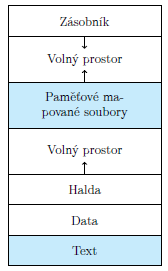
\includegraphics[scale=1]{images/mem_page_file.png}
	\caption{Paměťově mapovaný soubor}
	\label{mem_page_file}
\end{figure}

\emph{Anonymní stránky} jsou stránky co nejsou svázané se souborem a~jsou odkládány do~speciálního \emph{odkládacího souboru} (\emph{swap file}) na~\emph{odkládacím oddílu} (\emph{swap partition}) souborového systému. Jedná se o~data z~haldy a~zásobníku.

\begin{figure}[ht]
	\centering
	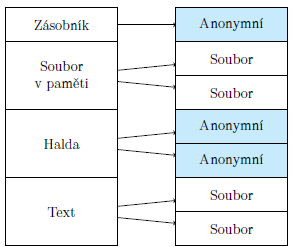
\includegraphics[scale=1]{images/mem_page_anon.png}
	\caption{Anonymní stránky}
	\label{mem_page}
\end{figure}

\subsection{Algoritmus LRU: Least Recently Used}

Nedávno používané stránky budou patrně použity znovu a~ty starší pravděpodobně ne. Z~tohoto důvodu je třeba udržovat pořadový seznam všech stránek v~hlavní paměti podle jejich doby použití. Na~začátku je naposledy použitá stránka a~na konci nejdéle nepoužitá. Seznam se navíc aktualizuje při~každém použití stránky. Pro~rychlé provedení algoritmu se využívá hardware.

Jedna z~možností je použití hardware s~64bitovým čítačem, který je inkrementován po~vykonání každé instrukce. Každá stránka má přiděleno jedno návěští kde je hodnota čítače. Po~použití stránky se do~návěští uloží aktuální hodnota čítače. Když je potřeba odstranit stránku je vybrána ta s~nejnižší hodnotou čítače, jelikož byla nižší hodnota čítače znamená, že již proběhlo mnoho instrukcí $\rightarrow$ stará stránka.

\clearpage

Druhá možnost spočívá ve~využití matic (opět v~hardware). Pro~$n$ možných stránek ve~FAP je použita matice $n \times n$ bitů. Při~každém použití stránky $k$ se nastaví bity řádku $k$ na~1 a~poté se vynuluje sloupec $k$. Řádek s~nejnižší binární hodnotu patří stránce nejdéle nepoužité a~je tedy vybrán%
\footnote{Skripta na~straně 72 mají pěkný příklad.}%
.

\subsection{Algoritmus NFU: Not Frequently Used}

NFU je softwarové řešení, které také využívá čítače. Pro~každou stránku je udržován bit A (accessed), který je nastaven kdykoliv je daná stránka použita. Toto je monitorováno v~intervalech daných přerušením od~hodin, každý interval jsou všechny stránky prohledány a~hodnota bitu A je přidána k~čítači. 0 se přidává pokud ke~stránce nebylo přistoupeno, 1 pokud bylo. Algoritmus vybírá stránku s~nejnižší hodnotou čítače (stránka není často používána).

Nevýhodou klasického NFU je fakt, že nikdy nenuluje hodnoty, preferuje tedy dříve často využívané stránky. Tento problém \emph{stárnutí stránek} modifikovaný algoritmus. Před přičtením hodnoty bitu A k~čítači provede bitový posun o~1bit do~prava (prakticky dělení dvěma). Následně je bit A přičten k~bitu s~nejvyšší váhou (MSB, \emph{Most Significant Bit}). U~klasického NFU to byl LSB (\emph{Least Significant Bit}).

Nedostatky této modifikace:

\begin{itemize}
	\item Pokud má dojít k~rozhodnutí mezi dvěma stránkami, vždy se vybere ta stránka s~menší hodnotou čítače. Nemáme však záruku že se jedná o~nejdéle nepoužitou stránku.
	\item Čítače mají omezený počet bitů, po~určitém čase mohou být všechny bity vynulované, pak nelze říct jestli byla stránka využita před $n+1$ intervaly (kde $n$ je počet bitů čítače) nebo před 100 intervaly. Stránky jsou pak vybrány náhodně.
\end{itemize}

%%%%%%%%%%%%%%%%%%%%%
% SOUBOROVÉ SYSTÉMY %
%%%%%%%%%%%%%%%%%%%%%

\clearpage
\section{Souborové systémy -- organizace dat na~paměťovém úložišti, metody ukládání datových bloků}

Souborový systém definuje jak jsou organizovaná data uložena na~paměťovém médiu, a~to jak vestavěném, tak externím. Data jsou organizována ve~formě souborů, které se potom sdružovány do~adresářů%
\footnote{Adresářová struktura bývá poskádána hierarchicky. Pro~jednouživatelské systémy se užívá \emph{plochý} systém, kde je jeden adresář a~v něm všechny soubory.}%
.

Souborové systémy udržují informace o~umístění dat jednotlivých souborů na~paměťovém médiu. Mimo to mohou poskytovat i~časové informace (vytvoření a~modifikace souboru). Ve víceuživatelských systémech se uchovávají i~informace o~\emph{vlastnících} a~\emph{přístupových právech} k~souboru. Informace o~souboru dělíme na~data a~metadata:

\begin{itemize}
	\item data -- obsah souboru.
	\item metadata -- data potřebná pro~práci se soubory jako informace o~umístění, časová informace nebo přístupová práva.
\end{itemize}

Paměťová média se typicky rozdělují na~několik samostatných částí. První je \emph{MBR} (\emph{Master Boot Record}) obsahující zavaděč operačního systému, identifikátor disku a~tabulku oddílů (\emph{partition table}) a~může obsahovat i~další části. MBR zavaděč je spouštěn kódem v~BIOS (\emph{Basic Input-Output System}). Úkolem zavaděče je načíst zaváděcí sektor z~aktivního oddílu, ten obsahuje operační systém který se spustí%
\footnote{Zaváděcí sektor se liší podle OS}%
.

\begin{figure}[ht]
	\centering
	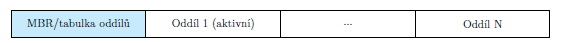
\includegraphics[scale=1]{images/mem_partitions.png}
	\caption{Oddíly disku}
	\label{mem_partitions}
\end{figure}

V~tabulce oddílů jsou uloženy informace o~umístění jednotlivých oddílů, tedy kde začínají a~kde končí. Na~oddílech se mohou vyskytovat různé souborové systémy a~na těch pak OS.

\subsection{Datové bloky}

Souborové systémy ukládají soubory do~tzv. \emph{datových bloků} (\emph{fragmentů}). Důležité je jak velký jeden blok je, jelikož velké bloky mohou podléhat \emph{interní fragmentaci} z~důvodu, že je soubor nenaplní a~\emph{datový blok} je nejmenší jednotka souborového systému. Naopak velmi malé bloky zpomalují operace se soubory, jelikož každý blok vyžaduje vyhledání jeho umístění.

\subsubsection{Kontinuální ukládání bloků}

Bloky jsou ukládány na~paměťovém médiu za~sebou. Tento způsob je vhodný u~plotnových disků, jelikož minimalizuje přesun čtecích hlav (mimo přesun hlav mezi cylindry). Záznam adresářů udržuje jen počáteční adresu souboru a~počet bloků (tj. jeho velikost). Problém vzniká při~rozšiřování souborů nebo zmenšování souborů.

Navíc dochází k~\emph{externí fragmentaci} skrz změny ve~velikostech souborů vznikají volné oblasti mezi záznamy, které však nejsou dostatečně velké pro~jakýkoliv soubor.

Procesu odstranění tohoto problému se říká \emph{defragmentace}. Všechny využité bloky se přesunou na~jiný filesystem, původní data se smazána a~poté se přesunou zpět. Jde o~časově náročnou operaci, kterou je třeba provádět periodicky.

\subsubsection{Ukládání bloků nesouvisle s~ukazateli v~bloku}

Bloky nejsou na~médiu rozděleny souvisle, místo toho je část jejich prostoru obětován ukazateli na~další blok souboru. Při~vytvoření souboru je nalezen volný blok kdekoliv na~paměťovém médiu a~je použit pro~nová data\footnote{Pokud má soubor nulovou velikost je ukazatel nastaven jako neplatný.}. Takto prakticky funguje jako \emph{linked list} a~nenastává problém s~externí fragmentací.

Avšak přesně tento přístup je nevýhodou této možnosti. Při~čtení je potřeba nejprve načíst první blok a~postupně hledat bloky pomocí ukazatelů. Každé načtení je tedy z~jiného sektoru disku a~zpomaluje program. Další problém je, že ukazatel ubírá místo z~bloku. Řešením pro~tento problém je seskupit bloky a~zavést ukazatel na~ně, pointer pak zabírá menší procenty paměti a~urychluje se práce s~daty. Bohužel ale dochází k~\emph{interní fragmentaci}\footnote{Existuje i~možnost poškození ukazatele, pokud se jedná o~první ukazatel tak se přijde o~celý soubor.}.

\subsubsection{Ukládání bloků nesouvisle s~ukazateli v~indexačním bloku}

Ukazatele nejsou obsaženy v~samotném bloku, ale v~tabulce ukazatelů pro~daný soubor, kterou udržuje ukazatel v~adresáři souboru. Při~vytvoření jsou všechny ukazatele neplatné, při~zápisu dat do~volných bloků se postupně aktualizují.

Nedochází sice k~externí fragmentaci, ale k~plýtvání paměti. Pokud se vytvoří malý soubor tak bude zabrán jeden celý blok navíc pro~udržování indexační tabulky, který se však nezaplní. Proto je třeba vhodně volit velikost tabulky.

Přístupy pro~práci s~indexačními bloky:
\begin{itemize}
	\item Přímé odkazy -- indexační blok obsahuje ukazatele na~datové bloky, v~případě velkého souboru lze propojit více indexačních bloků, poslední ukazatel je tedy buď neplatný (pro malé soubory) nebo ukazuje na~začátek další tabulky.
	\item Nepřímé odkazy -- indexační blok obsahuje odkazy na~další indexační bloky, které obsahují přímé odkazy na~datové bloky. Pro~přístup k~blokům se nejprve načte indexační blok přes nepřímý odkaz a~až poté se načte blok přes přímý odkaz.
	\item Kombinace -- Indexační blok obsahuje přímé i~nepřímé a~dokonce i~zanořené nepřímé odkazy, tedy nepřímý odkaz na~nepřímý odkaz. Je vhodný pro~velké soubory (nepřímé odkazy s~několika úrovněmi) i~pro~malé soubory (přímé odkazy).
\end{itemize}

\begin{figure}[ht]
	\centering
	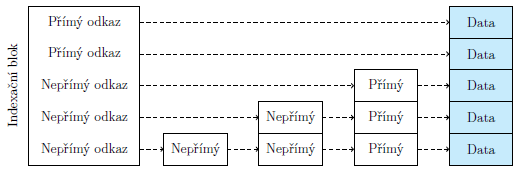
\includegraphics[scale=1.2]{images/mem_block_index.png}
	\caption{Indexační blok}
	\label{mem_block_index}
\end{figure}

\subsection{Ukládání dat a~metadat na~HDD}

Pevný disk se skládá z~ploten\footnote{Pro čtení z~ploten se používá více hlav.} (které jsou uspořádány nad sebou), které jsou rozděleny na~stopy a~ty zase na~sektory. Sektor je nejmenší jednotka pro~ukládání dat na~pevném disku. Datové bloky souborových systémů, mohou zabírat jeden nebo více sektorů. Při~práci s~daty se nejprve načtou metadata o~souboru (přístupová práva a~o uložení dat), tedy hlavice musí přejít na~pozici metadat a~až poté na~pozici dat\footnote{Přilíž velkému množství přesunů se zamezuje pomocí organizace do~tzv. \emph{cylindrů}, což je sada nad sebou umístěných stop. Tyto společně udržují data a~metadata.}.

\begin{figure}[ht]
	\centering
	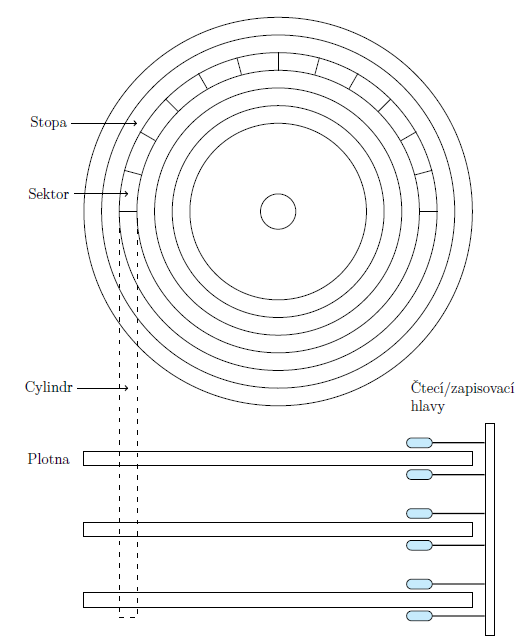
\includegraphics[scale=1]{images/mem_hdd.png}
	\caption{Dělení paměťových bloků na~HDD}
	\label{mem_hdd}
\end{figure}

%%%%%%%%%%%%%%%
% KONZISTENCE %
%%%%%%%%%%%%%%%

\clearpage
\section{Konzistence dat -- data a~metadata, žurnálovací souborové systémy}

Když se v~souborovém systému pracuje s~daty (zapisování a~mazání), může dojít k~situaci kdy se data dostanou do~nekonzistentního stavu, z~důvodu pádu systému. Nekonzistentními situacemi mohou být:

\begin{itemize}
	\item Soubor nebyl smazán, i~když k~tomu byl zadá požadavek.
	\item Část dat byla aktualizována zápisem, další část ne.
\end{itemize}

Jak probíhá mazání souboru?

\begin{enumerate}
	\item Odstranění záznamu o~souboru z~adresáře,
	\item uložení čísla i-uzlu (viz dále) souboru do~seznamu volných i-uzlů,
	\item uložení datových bloků souboru do~seznamu volných bloků k~použití.
\end{enumerate}

Pokud dojde k~pádu systému mezi kroky 1 a~2, tak zůstane i-uzel v~použitém stavu i~když tomu tak není. Tato skutečnost plýtvá pamětí, jelikož i-uzel nemůže být využit pro~jiná data. Podobná situace nastává při~pádu mezi kroky 2 a~3. Jako řešení tohoto problému byly navrhnuty žurnálovací systémy.

\subsection{Ukládání metadat}

Metadata se ukládají ve~speciální struktuře, zvané \emph{i-uzel} (tj. \emph{i-node})%
\footnote{Detaily budou specifické pro~OS Linux} %
. Tyto struktury obsahují metadata o~souboru jako typ souboru, vlastník, skupina vlastníka, přístupová práva, délka souboru, čas vytvoření, čas posledního přístupu a~čas modifikace. Dále i-uzel obsahuje ukazatele na~bloky souboru.

V~adresářích se vyskytují položky obsahující jméno souboru a~číslo relevantního \emph{i-uzlu}. Tyto informace jsou důležité pro~nalezení souborů. Navíc může být v~různých adresářích více souborů se stejným jménem ukazující na~jeden soubor/\emph{i-uzel} (tj. \emph{pevné odkazy}/\emph{hard link})%
\footnote{Při~smazání pevného odkazu je počet těchto odkazů snížen o~jedno. Pokud je počet roven 0 je soubor definitivně smazán.}%
.

Dále existuje \emph{symbolický odkaz} (\emph{symlink}), kdy soubor odkazuje na~jiný. Při~smazání souboru, na~který \emph{symlink} odkazuje, nedochází ke~smazání souboru se symbolickým odkazem.

\subsection{Žurnálovací souborové systémy}

Ve~svém \enquote{žurnálu} udržují záznamy o~plánovaných změnách před jejich provedením. Pokud dojde k~pádu systému, je schopen dostat data a~metadata do~konzistentního stavu pomocí předešle uložených plánů operací v~žurnálu. Uložená operace je však proveditelná pouze pokud je kompletně uložená.

Pokud není operace zapsána jako celek do~žurnálu před pádem systému, je ignorována. Kontrolu lze provádět pomocí kontrolního součtu, v~případě pádu systému před kompletním zápisem do~žurnálu nebude součet sedět a~zápis bude ignorován.

Do~žurnálu lze ukládat pouze metadata nebo metadata a~vlastní data souboru. První varianta je rychlejší ale s~možností ztráty konzistence, u~druhé možnosti je to naopak.

\begin{itemize}
	\item Při~ukládání pouze metadat může dojít k~inkonzistenci mezi metadaty. Např. při~přidání dat do~souboru:
	\begin{enumerate}
		\item Změna záznamu o~velikosti souboru v~jeho i-uzlu (metadata).
		\item Z volných datových bloků je vybrán prostor pro~nová data (metadata).
		\item Do vybraných bloků jsou zapsány data (data).
	\end{enumerate}
	Pokud dojde k~pádu systému před třetím krokem, budou v~žurnálu zaznamenány datové bloky, ale v~těch bude náhodná změť paměti.
	\item Při~ukládání s~daty souborů jsou do~žurnálu ukládány kopie všech datových bloků do~kterých se bude zapisovat. Pokud dojde k~pádu, je operace zápisu provedena znovu nad kopií datových bloků. To značně zpomaluje operaci zápisu. Využívá se pouze v~systémech, kde vyžadujeme naprostou ochranu dat.
\end{itemize}

Základní implementace:

\begin{enumerate}
	\item Kopie žurnálu mohou být umístěny na~různých paměťových médiích za~účelem zálohování v~případě poruchy jiného média.
	\item Plánované změny v~žurnálu mohou být dále ukládány v~jiném žurnálu z~důvodu zvýšení redundance.
	\item Žurnál je ukládán na~stejném nebo jiném médiu, z~důvodu vyšší rychlosti.
\end{enumerate}

%%%%%%%%%%%%%%
% NETWORK OS %
%%%%%%%%%%%%%%

\clearpage
\section{Síťová část OS -- stavy soketů při~komunikaci, síťová systémová volání, serverové procesy}

Socket je vstupně výstupní bod do~sítě zahrnující adresu síťové i~transportní vrstvy. Pomocí IP adresy specifikuje koncovou stanici a~pak s~portem v~kombinaci s~protokolem cílovou službu stanice. Sokety na~straně klienta a~serveru vytvoří komunikační kanál k~přenosu dat.

\begin{figure}[ht]
	\centering
	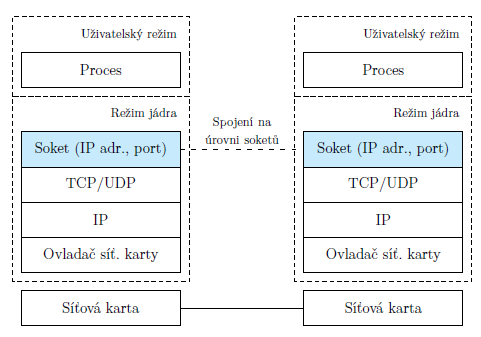
\includegraphics[scale=1]{images/network_socket.png}
	\caption{Síťové sockety}
	\label{network_socket}
\end{figure}

Při~realizaci síťové komunikace (v tomto případě spojově orientované TCP) procházejí sokety různými stavy: čekání, sestavování (SYN, ACK), přenos (PSH, ACK) a~ukončování (FIN, ACK).

Přechody mezi stavy soketů jsou řízeny příznaky v~záhlaví TCP segment. Příznak ACK signalizuje potvrzení přijatých dat, PSH přenos dat, SYN žádost o~sestavení spojení, FIN ukončení spojení.

\subsection{Stavy soketů}

\paragraph{Sestavení spojení}

První jednosměrné spojení se zahájí zasláním segmentu s~příznakem SYN, naslouchající soket na~straně serveru segment přijme a~potvrzuje žádost klienta zasláním segmentu s~příznakem ACK. Tento stejný segment zasílá žádost o~sestavení druhého jednosměrného spojení s~příznakem SYN. Třetí segment opět potvrzuje.

\begin{figure}[ht]
	\centering
	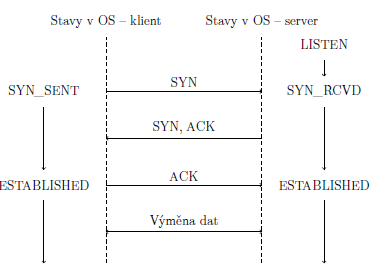
\includegraphics[scale=1]{images/network_three_handshake.png}
	\caption{Navázání TCP spojení}
	\label{network_three_handshake}
\end{figure}

Soket na~straně serveru může při~sestavování být ve~stavu LISTEN (naslouchá/čeká na~spojení) nebo SYN\_RCVD (první SYN segment přijat). Soket na~straně klienta může být ve~stavu SYN\_SENT (SYN segment zaslán). Po~navázání se přechází do~stavu ESTABLISHED.

\paragraph{Přenos dat}

TCP segmenty mají příznak PSH. Jako odpověď se opět zasílají segmenty s~příznakem ACK pro~potvrzení přijetí dat.

\paragraph{Ukončení spojení}

Spojení může ukončit jakákoliv strana zasláním segmentu s~příznakem FIN, ovšem pouze svoje jednosměrné spojení. Druhé zůstává otevřené a~může stále zasílat data, dokud jej druhá strana neukončí. Při~ukončování spojení prochází sokety těmito stavy:
\begin{itemize}
	\item FIN\_WAIT1 -- stav soketu stanice která jako první ukončila jednosměrné spojení (zasláním FIN).
	\item CLOSE\_WAIT -- stanice přijala segment s~příznakem FIN a~potvrzení bylo vysláno.
	\item FIN\_WAIT2 -- stanice obdržela potvrzení o~ukončení spojení, tento stav setrvává dokud druhá stanice také nepošle FIN.
	\item LAST\_ACK -- druhá stanice ukončuje druhé jednosměrné spojení (zasláním FIN).
	\item TIME\_WAIT -- stanice potvrzuje ukončení spojení, avšak typicky počká pár minut. Důvodem je fakt, že zaslané potvrzení se může ztratit, stanice si o~něj případně zažádá znovu.
	\item CLOSED -- potvrzení přijato a~spojení ukončeno.
\end{itemize}

\begin{figure}
	\centering
	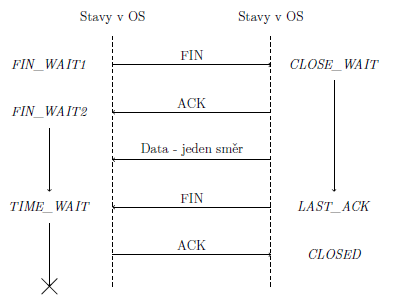
\includegraphics[scale=1]{images/network_tcp_close.png}
	\caption{Ukončení TCP spojení}
	\label{network_tcp_close}
\end{figure}

\subsection{Síťová systémová volání}

Správa soketů v~OS Linux se provádí pomocí systémových volání.

\begin{itemize}
\item \textbf{socket}: Založení nového soketu.
\item \textbf{connect}: Systémové volání na~straně klienta pro~navázání spojení se soketem na~straně serveru. Navazování spojení probíhá pomocí three-way handshake (viz obrázek \ref{network_three_handshake}).
\item \textbf{bind}: Přiřadí soketu IP adresu a~port na~straně serveru. Bez~zavolání by byl soket svázán s~náhodným portem z~dynamického rozsahu (49152-65535). U~serveru se ovšem očekává, že bude naslouchat na~portu svázaném se službou (FTP 21, SSH 22, HTTP 80, HTTPS 443, \dots). U~klienta je port generován z~dynamického rozsahu, toto volání se tedy nepoužívá.
\item \textbf{listen}: Převede soket na~straně serveru do~pasivního režimu kdy přijímá příchozí spojení (pomocí systémového volání accept). Vytvoří se vstupní fronta pro~příchozí spojení.
\item \textbf{accept}: Voláno na~straně severu k~vyzvednutí požadavku o~spojení ze~vstupní fronty. Volání vytvoří nový soket podle parametrů žádosti o~spojení. Pokud je accept zavolán v~době, kdy je vstupní fronta prázdná, spojení je zablokováno do~doby než žádost přijde.
\item \textbf{close}: Uzavírá soket. Ukončení spojení zmíněno dříve.
\item \textbf{write}, \textbf{read}: Systémová volání pro~přenos dat. Data jsou přenášena s~dříve zmíněnými příznaky segmentů PSH a~ACK.
\end{itemize}

\subsection{Serverové procesy}

Jedná se o~síťové služby, které jsou zprostředkovány programy (tj. \emph{servery}). Proces každého serveru má přiřazenou adresu -- port, ta rozlišuje jednotlivé servery v~rámci jedné stanice\footnote{Servery pracující na~pozadí označujeme jako \emph{démony} (\emph{daemon})}. Servery lze spouštět dvojím způsobem: stále (při~startu systému) nebo na~požádání (pouze když je potřeba).

Stále spuštěné servery typicky musí reagovat rychle a~obsluhují velké množství žádostí. Naopak u~serverů na~vyžádání se předpokládá méně časté využití, proto je spouští tzv. \emph{superserver/superdémon} (jeden ze~stále běžících serverů)%
\footnote{Je třeba se správně rozhodnout jak servery rozdělit. Stále běžící permanentně ubírají systémové prostředky, zatímco servery na~vyžádání budou reagovat se zpožděním při~zahájení komunikace.}%
.

\begin{figure}[ht]
	\centering
	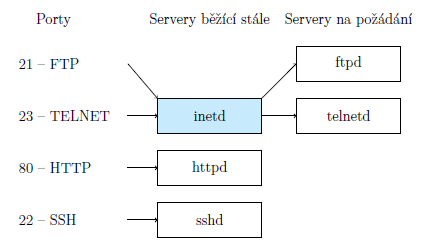
\includegraphics[scale=1]{images/network_server_proc.png}
	\caption{Serverové procesy}
	\label{network_server_proc}
\end{figure}

Příklad použití superserveru lze vidět na~obrázku \ref{network_server_proc}. Superserver \textbf{inetd} běží stále a~naslouchá na~\textbf{FTP} a~\textbf{TELNET} portech (21 resp. 23). V~případě, že přijde požadavek na~jeden z~těchto prostů aktivuje superserver korespondující server. Servery \textbf{httpd} (HTTP) a~\textbf{sshd} (SSH) jsou svázány přímo s~portem a~běží stále.
